\documentclass[epsfig,10pt,fullpage]{article}

\newcommand{\LabNum}{3}
\newcommand{\CommonDocsPath}{../../../../common/docs}
\input{\CommonDocsPath/preamble.tex}

\begin{document}
~\\
\centerline{\huge Laboratory Exercise 3}
~\\
\centerline{\large Memory-Mapped I/O, Polling and Timers}
~\\

\noindent
The purpose of this exercise is to explore the use of devices that provide input and
output capabilities for a processor. We assume that you are using the Nios~V processor in
the DE1-SoC Computer. A good approach is to first implement each part of this exercise by 
using the {\it CPUlator} simulator, and then to implement your solution in a hardware board,
if available.  If a hardware system other than the DE1-SoC Computer is being used, then 
some parts of this exercise may need to be modified to suit the features of your board. 

~\\
\noindent
There are two basic techniques for synchronizing with I/O devices:
program-controlled \emph{polling} and \emph{interrupt-driven} approaches.  
We will use the polling approach in this exercise, writing programs in the Nios~V
assembly language.  {\it Parallel port} interfaces, as well as a {\it timer} hardware 
module, will be used as examples of I/O hardware.

~\\
\noindent
In general, a {\it parallel port} provides for data transfer in either the input or 
output direction.  The transfer of data to/from the processor is done in parallel and may 
involve from 1 to 32 bits.  The number of bits, $n$, and the type of transfer depend on the
specific parallel port being used. The parallel port interface can contain the four 
registers shown in Figure~\ref{fig:parallel}.

\begin{figure}[htb]
	\begin{center}
	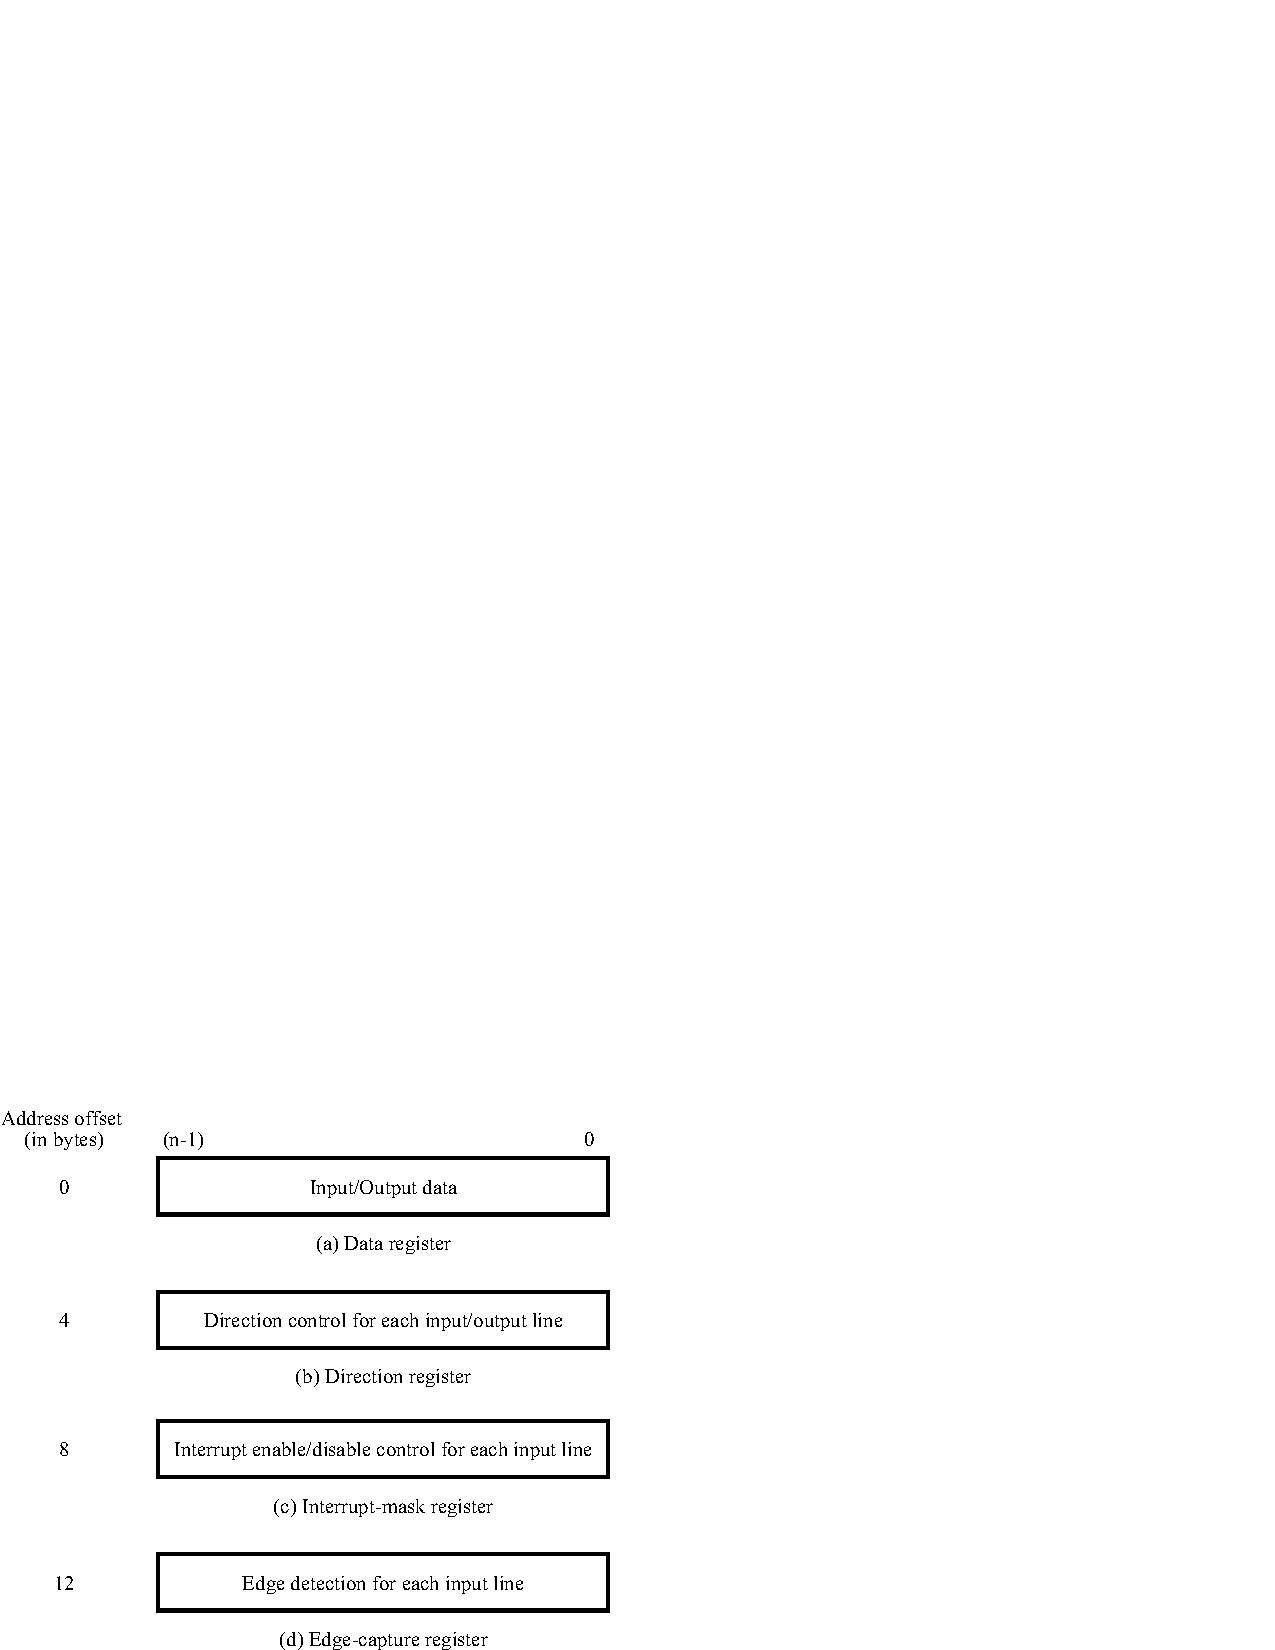
\includegraphics[scale=0.90]{figures/figureparallel.pdf}
	\end{center}
	\caption{Registers in the parallel port interface.}
\label{fig:parallel}
\end{figure}

\noindent
Each register is $n$ bits long. The registers have the following purpose:
\begin{itemize}
\item {\it Data} register: holds the $n$ bits of data that are transferred between the parallel 
port and the Nios~V processor. The {\it Data} register can be implemented as an input, output,
or a bidirectional port.
\item {\it Direction} register: defines the direction of transfer for each of the $n$
data bits when a bidirectional interface is generated.
\item {\it Interrupt-mask} register: used to enable interrupts from the
input lines connected to the parallel port. This register will be described in more detail
in a later laboratory exercise. 
\item {\it Edge-capture} register: indicates when a change of logic value is detected in 
the signals on the input lines connected to the parallel port. Once a bit in the edge
capture register becomes asserted, it will remain asserted. An edge-capture bit can be
de-asserted by writing to it using the Nios~V processor.
\end{itemize}
\noindent
Not all of the registers depicted in Figure~\ref{fig:parallel} are present in some 
parallel ports. For example, the {\it Direction} register is included only when a 
bidirectional interface is present in the parallel port.
The {\it Interrupt-mask} and {\it Edge-capture} registers must be included if
interrupt-driven input/output (described in a later laboratory exercise) is used.

~\\
The parallel port registers are memory mapped, starting at a specific {\it base} address.
The base address becomes the address of the {\it Data} 
register in the parallel port. The addresses of the other three registers have offsets 
of 4, 8, or 12 bytes (1, 2, or 3 words) from this base address. In the DE1-SoC Computer parallel 
ports are used to connect to several types of hardware resources, including {\it SW} slide 
switches, {\it KEY} pushbuttons, {\it LEDs}, and seven-segment displays.
~\\
~\\
{\bf Conforming to the Nios~V Procedure Call Standard}
\\
\\
\noindent
The Nios~V {\it Procedure Call Standard} (PCS) provides guidelines (``rules'') for how registers
should be used in a program, especially when subroutines are involved. The PCS states that
parameters should be passed to a subroutine by using the Nios~V {\it argument} registers
{\it a0} to {\it a7}. Results should be returned from a subroutine in registers 
{\it a0} and {\it a1}. The PCS states that a subroutine can freely modify the Nios~V
{\it temporary} registers {\it t0} to {\it t6}, but it is not permitted to have changed the 
contents of the Nios~V {\it save} registers {\it s0} to {\it s11} after execution of the subroutine.
If these save registers need to be changed, then the register values should first be saved to
memory and later restored before returning from the subroutine. (Note: if you are using 
{\it CPUlator}, then you will see an error stating 
that you have ``clobbered'' one ore more of registers {\it s0} to {\it s11} if you over-write
these registers in a subroutine without saving/restoring their values as required by the PCS.)

~\\
\noindent
You should always follow the Nios~V PCS in all assembly-language code that you write.

\subsection*{Part I}

\noindent
The DE1-SoC Computer contains several parallel ports that are connected to simple switches,
lights, and displays. Figure~\ref{fig:LED} depicts the parallel port connected to the ten
red lights, called {\it LEDR}, on the DE1-SoC board. Software code can turn the lights on 
or off by writing the value 1 or 0, respectively, to each of the ten bit-positions in the 
register that is mapped to address \texttt{0xFF200000}. 

\begin{figure}[htb]
	\begin{center}
	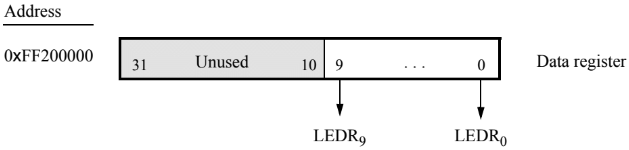
\includegraphics[scale=.55]{figures/figureLEDR.png}
	\end{center}
	\caption{The parallel port connected to the red lights {\it LEDR}.}
\label{fig:LED}
\end{figure}

\noindent
The parallel port connected to the ten slide switches, called {\it SW}, on the DE1-SoC
board is shown in Figure~\ref{fig:SW}. Software code can load the state of the switches by
reading from the register mapped to address \texttt{0XFF200040}.

\begin{figure}[htb]
	\begin{center}
	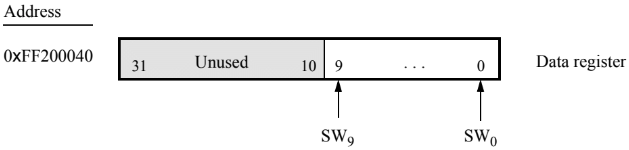
\includegraphics[scale=.55]{figures/figureSW.png}
	\end{center}
	\caption{The parallel port connected to the {\it SW} switches.}
\label{fig:SW}
\end{figure}

~\\
The DE1-SoC Computer has two parallel ports connected to the seven-segment 
displays on the DE1-SoC board. The port connected to the displays {\it HEX}$\,$3-0 is memory 
mapped at the base address {\sf 0xFF200020} and the other parallel port is connected to 
{\it HEX}$\,$5-4, at the base address {\sf 0xFF200030}. 
Figure~\ref{fig:HEX} shows how the display segments are connected to the parallel ports.  

\begin{figure}[htb]
	\begin{center}
	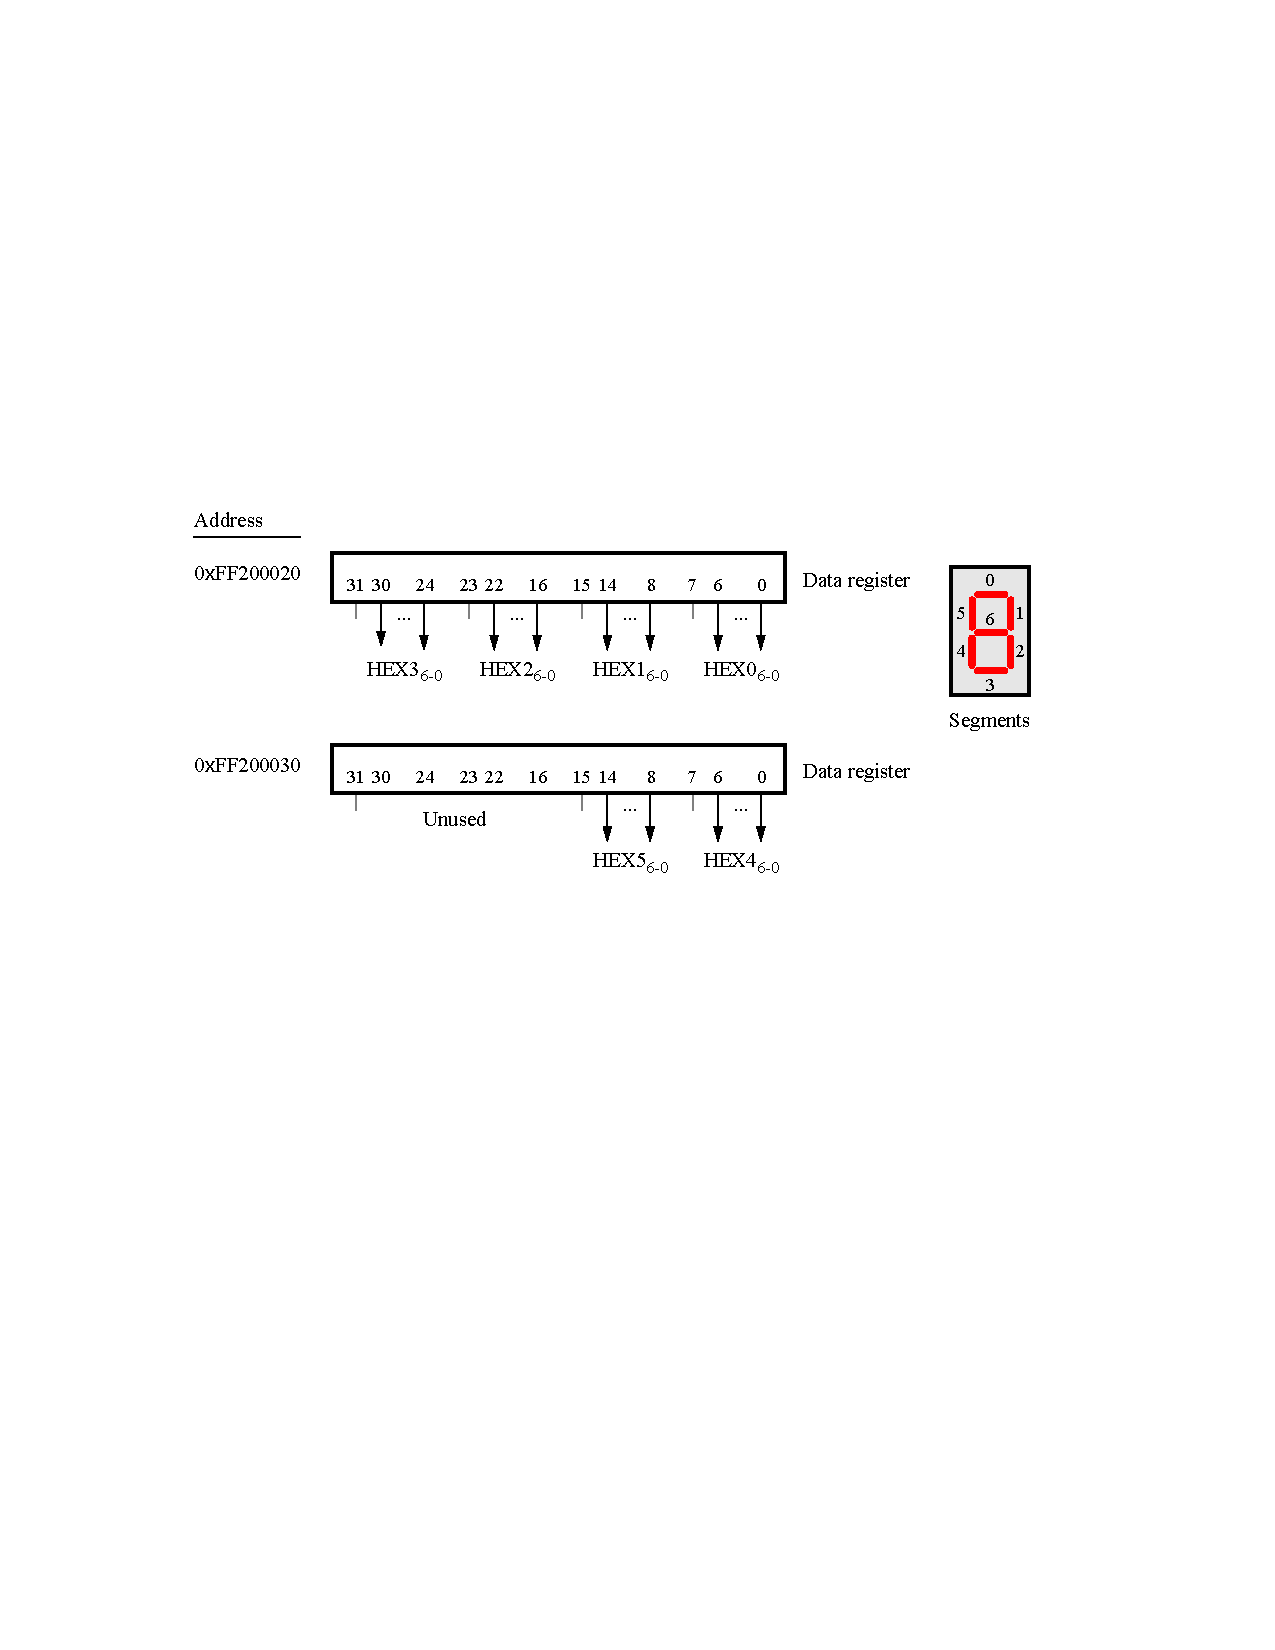
\includegraphics[scale=1]{figures/figureHEX.pdf}
	\end{center}
	\caption{The parallel ports connected to the seven-segment displays {\it HEX}$\,$5-0.}
\label{fig:HEX}
\end{figure}

~\\
\noindent
An example of code that uses the {\it LEDR}, {\it SW}, and {\it HEX}$\,$3-0 parallel ports is 
given in Figure~\ref{fig:SWHEX}. This code reads from the {\it SW} switches and writes the
resulting value to both the {\it LEDR} and {\it HEX}$\,$3-0 ports. Compile and execute
this code to experiment with different settings of the {\it SW} switches, and observe the
{\it LEDR} and {\it HEX}$\,$3-0 displays.

\begin{figure}[H]
\begin{center}
\lstinputlisting[style=defaultNiosVStyle]{../design_files/part1.s}
\end{center}
\caption{Assembly-language program that uses the parallel ports.}
\label{fig:SWHEX}
\end{figure}

\subsection*{Part II}

\noindent
You are to write a Nios~V program that displays a hexadecimal digit 
(\red{0}, \red{1}, $\ldots$, \red{9}, \red{A}, \red{b}, \red{C}, \red{d}, \red{E}, \red{F}) on the 
seven-segment display {\it HEX}0 as described below. The other seven-segment 
displays {\it HEX}$5-1$ should be set to be blank.  

~\\
\noindent
The following functionality should be included:

\begin{itemize}
\item If {\it KEY}$_0$ is pressed on the board, you should set the number displayed on 
{\it HEX}0 to \red{0}. 
\item If {\it KEY}$_1$ is pressed then you should increment the displayed number, 
but don't let the number go above \red{f} (i.e. pressing the key won't change the value if 
it is already at \red{f}$\,$).
\item If {\it KEY}$_2$ is pressed then decrement the number, but don't
let the number go below \red{0} (i.e. pressing the key won't change the value if it is
already \red{0}$\,$). 
\item Pressing {\it KEY}$_3$ should 
blank the display, and pressing any other KEY after that should return the display to~\red{0}.
\item
The parallel port connected to the pushbutton {\it KEYs} has the base address
{\sf 0xFF200050}, as illustrated in Figure~\ref{fig:KEY}. In your program, use 
the \emph{polling} I/O method to read the {\it Data} register to see when a button 
is being pressed. 
\item When you are not pressing 
any {\it KEY} the {\it Data} register provides~0, and when you press {\it KEY}$_i$ the 
{\it Data} register provides the value 1 in bit position $i$. Once a button-press is detected,
be sure that your program waits until the button is released. You \emph{must not} use the 
{\it Interruptmask} or {\it Edgecapture} registers for this part of the exercise.
\end{itemize}

\noindent
Implement your code in a file called {\it part2.s}. Compile and execute your code and test
it thoroughly according to the above specification. 

~\\
\begin{figure}[h]
	\begin{center}
	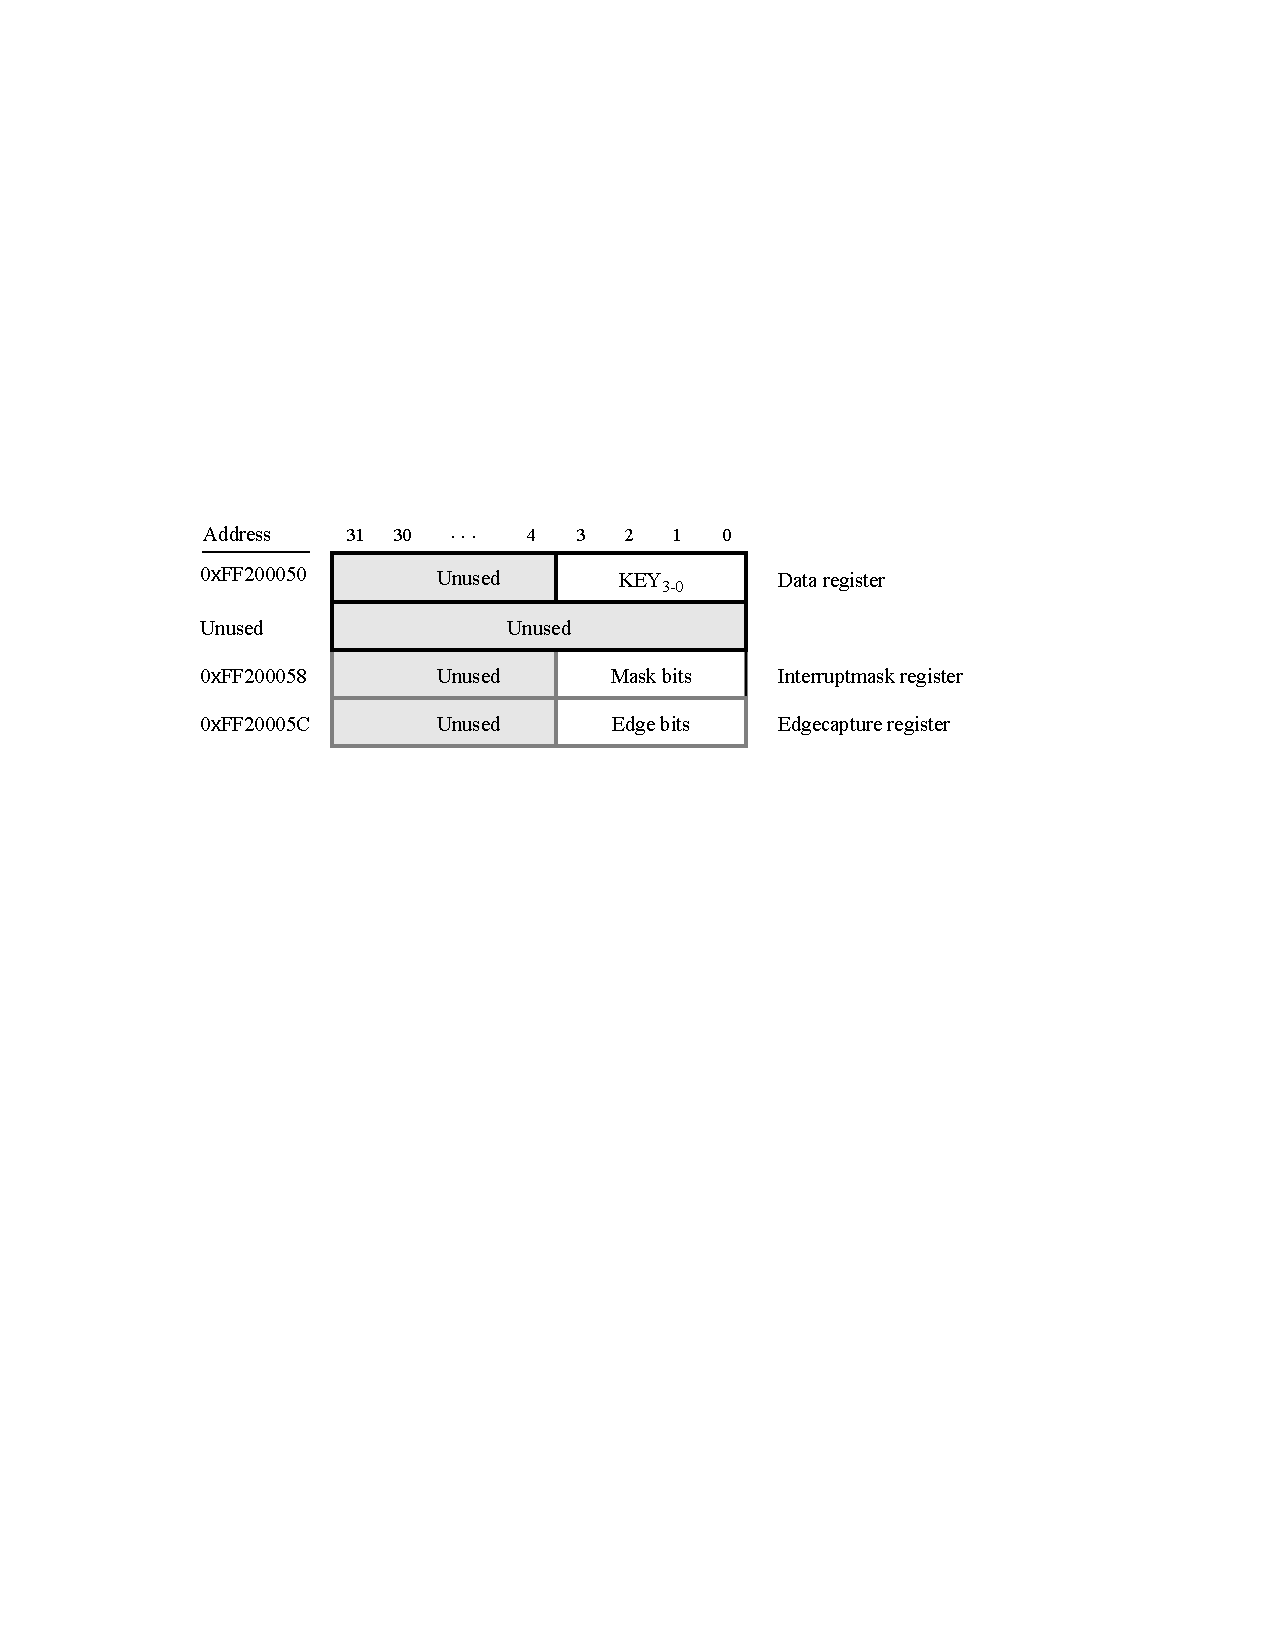
\includegraphics[scale=1]{figures/figureKEY.pdf}
	\end{center}
	\caption{The parallel port connected to the pushbutton {\it KEYs}.}
\label{fig:KEY}
\end{figure}

\subsection*{Part III}

\noindent
Write a Nios~V assembly language program that displays a two-digit hexadecimal \emph{counter} 
on the seven-segment displays {\it HEX}$\,$1-0. The counter should be incremented approximately
every one second. When the counter reaches the value \red{FF}, it should start again at
\red{00}.

~\\
\noindent
To achieve a delay of approximately one second, use a delay-loop in your assembly language
code. A suitable example of such a loop is shown below, which gives a good value for the delay 
when using the simulated Nios~V processor in the {\it CPUlator} tool. If you are using the
real Nios~V processor on a DE1-SoC board, then a much smaller delay value has to be used, 
because the Nios~V processor executes code {\it much} more quickly in hardware than in the
{\it CPUlator} simulation. 

~\\
\noindent
\begin{lstlisting}[style=defaultNiosVStyle]
delay:      li      t0, 15000000        # wait for a little while
dloop:      addi    t0, t0, -1
            bnez    t0, dloop
\end{lstlisting}

~\\
\noindent
To avoid ``missing'' any button presses while the processor is executing the delay loop, you
should use the {\it Edgecapture} register in the {\it KEY} port, shown in Figure~\ref{fig:KEY}.
When a pushbutton is pressed, the corresponding bit in the {\it Edgecapture} register is
set to 1; it remains set until your program resets it back to 0. You reset an {\it
Edgecapture} bit by writing a 1 into the corresponding position of the register.

~\\
\noindent
Put your code into a file called {\it part3.s}, and test and debug your program.

\subsection*{Part IV}

\noindent
In Part III you used a delay loop to cause the Nios~V processor to wait for approximately one
second. The processor loaded a large value into a register before the loop, and then 
decremented that value until it reached 0.  In this part you are to modify your code so that a
{\it hardware timer} is used to measure an exact delay of one second. 

~\\
\noindent
The DE1-SoC Computer includes a number of hardware timers, but for this exercise you will
use only the {\it Machine Timer}, which is part of the Nios~V processor. As illustrated
in Figure~\ref{fig:timer} the Machine Timer comprises two 64-bit registers. 
The {\it mtimecmp} register is memory-mapped to address \texttt{0xFF202100}, and the 
{\it mtime} register is mapped to address \texttt{0xFF202108}. Since these registers are
64 bits in width, two Nios~V memory accesses are needed to access either register. The
Nios~V processor can interact with the Machine Timer two mains ways: using interrupts, or
using polled-I/O. In this exercise you will use the polled-I/O method.

~\\
\noindent
When using polled-IO, an easy way to interact with the Machine Timer is as follows. First, you
store a {\it timeout} value into the {\it mtimecmp} register. If this timeout value fits 
within a 32-bit unsigned number, then you can just store it into the low word of {\it mtimecmp}, 
at address \texttt{0xFF202100}, and set the high-word of {\it mtimecmp}, at 
address \texttt{0xFF202104}, to 0. The Machine Timer is always running, and its 
current value is reflected in the {\it mtime} register. The Machine Timer increments at
the rate of 100,000,000 cycles per second in the DE1-SoC Computer. Each time the
value of the {\it mtime} register reaches the value stored in the {\it mtimecmp} register, 
then a {\it timeout} has occurred. Once this happens, you can begin the next timeout period 
by resetting the value of the {\it mtime} register to 0.

~\\
\noindent
Store your code for this part of the exercise in a file called {\it part4.s}. It should be
the same as in Part III, except that you should initialize the {\it mtimecmp} and {\it
mtime} registers at the beginning of your code. Set the {\it mtimecmp} register so as
to generate a timeout every one second. 
In your program's main loop, poll on the value of the {\it mtime} register to wait for each 
timeout period, rather than decrementing a register as in Part III. Test and debug
your program.

~\\
\begin{figure}[htb]
	\begin{center}
	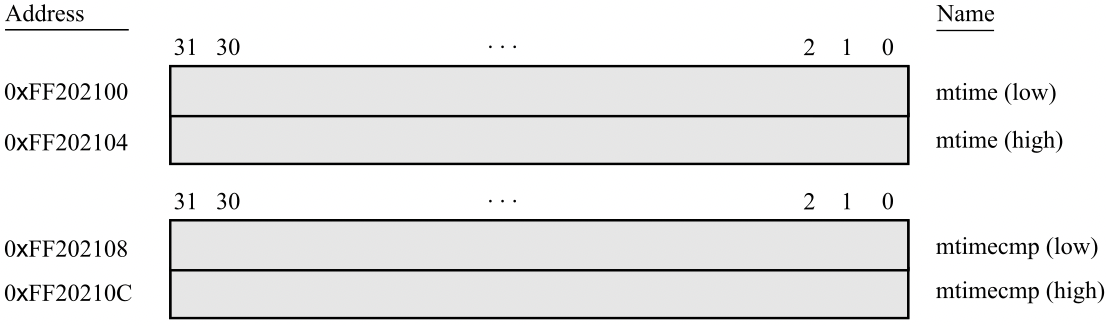
\includegraphics[scale=.55]{figures/figuretimer.png}
	\end{center}
	\caption{The Nios~V Machine Timer registers.}
\label{fig:timer}
\end{figure}

\input{\CommonDocsPath/copyright.tex}
\end{document}
\end{document}
